L'infrastruttura di comunicazione consiste tipicamente di sistemi SCADA con canali di comunicazione dedicati da e verso il centro di controllo del sistema e una Wide Area Network (WAN). I sistemi SCADA collegano tutte le principali strutture operative del sistema mentre la WAN è prevalentemente usata per azioni di mercato. Uno sviluppo importante per la Smart Grid (vedi Figura \ref{fig:cisg}) è quello di estendere la comunicazione a tutto il sistema di distribuzione e di stabilire una comunicazione bidirezionale con i clienti attraverso le Neighbourhood Area Network (NANs) che coprono le zone servite da sottostazioni di distribuzione. I clienti avranno la necessità di una Home Area Network (HAN) a cui saranno connessi smart device.
\begin{figure}[h]
	\centering
	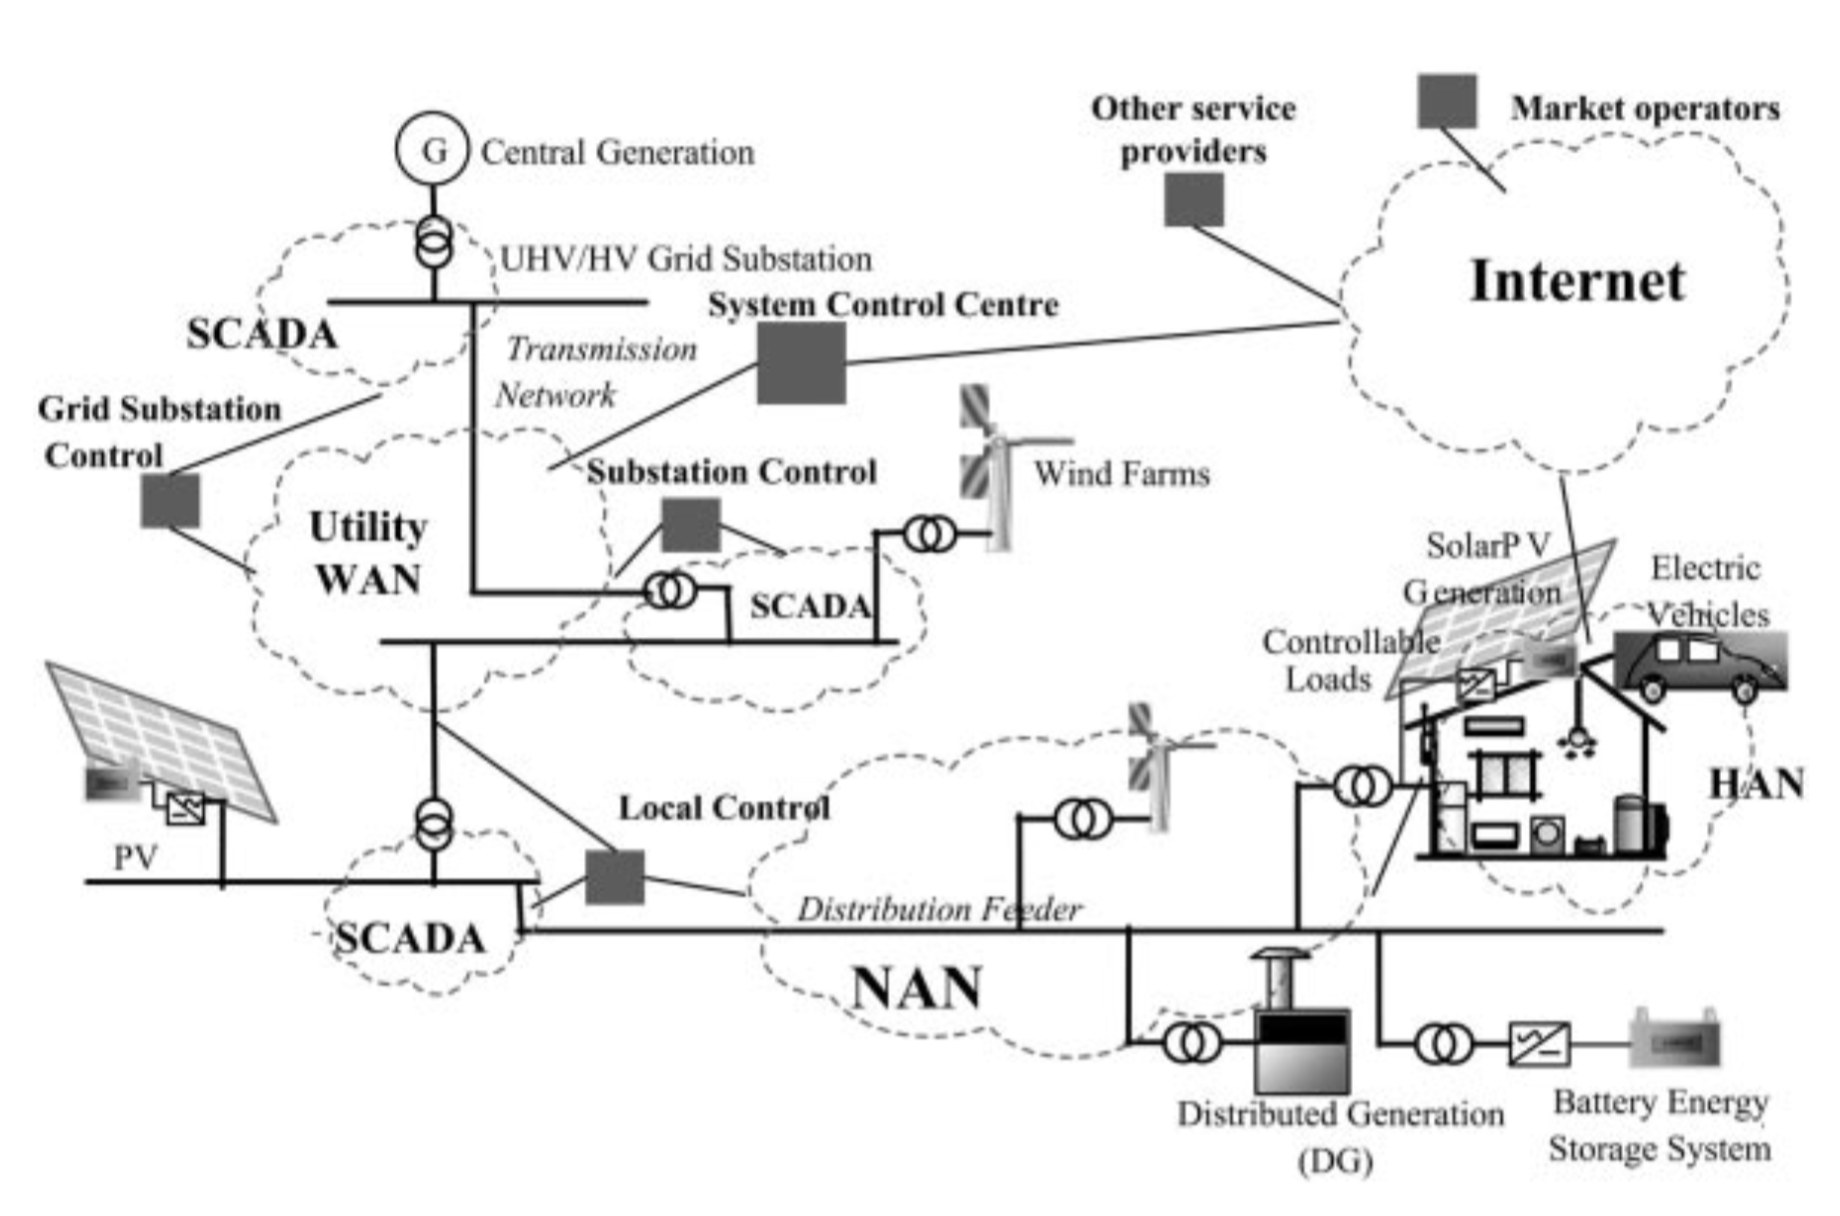
\includegraphics[scale=0.300]{imgs/comm_inf_SG.png}
	\caption{Una possibile infrastruttura di comunicazione per la Smart Grid} \label{fig:cisg}
\end{figure}\\
Le sotto-reti di comunicazione che andranno a comporre la Smart Grid utilizzano diverse tecnologie (vedi Figura \ref{fig:th}) e di particolare interesse è il modo in cui quest'ultime possono essere integrate in maniera efficace. Le Smart Grid possono utilizzare diverse tecnologie di comunicazione wired e wireless (ad esempio, cellulare , satellitare, microwave e WiMAX). Le tecnologie di comunicazione wireless short range, come WiFi e ZigBee,  possono essere utilizzate nelle HAN.
%Nel modello di riferimento ISO / OSI, gli strati superiori trattano applicazioni indipendentemente dal meccanismo di effettiva consegna mentre gli strati più bassi si occupano invio di informazioni indipendentemente dall' applicazione.
In questo capitolo, si descriveranno alcune tecnologie di comunicazione associate ai livelli inferiori del modello di riferimento ISO/OSI.
\begin{figure}[h]
	\centering
	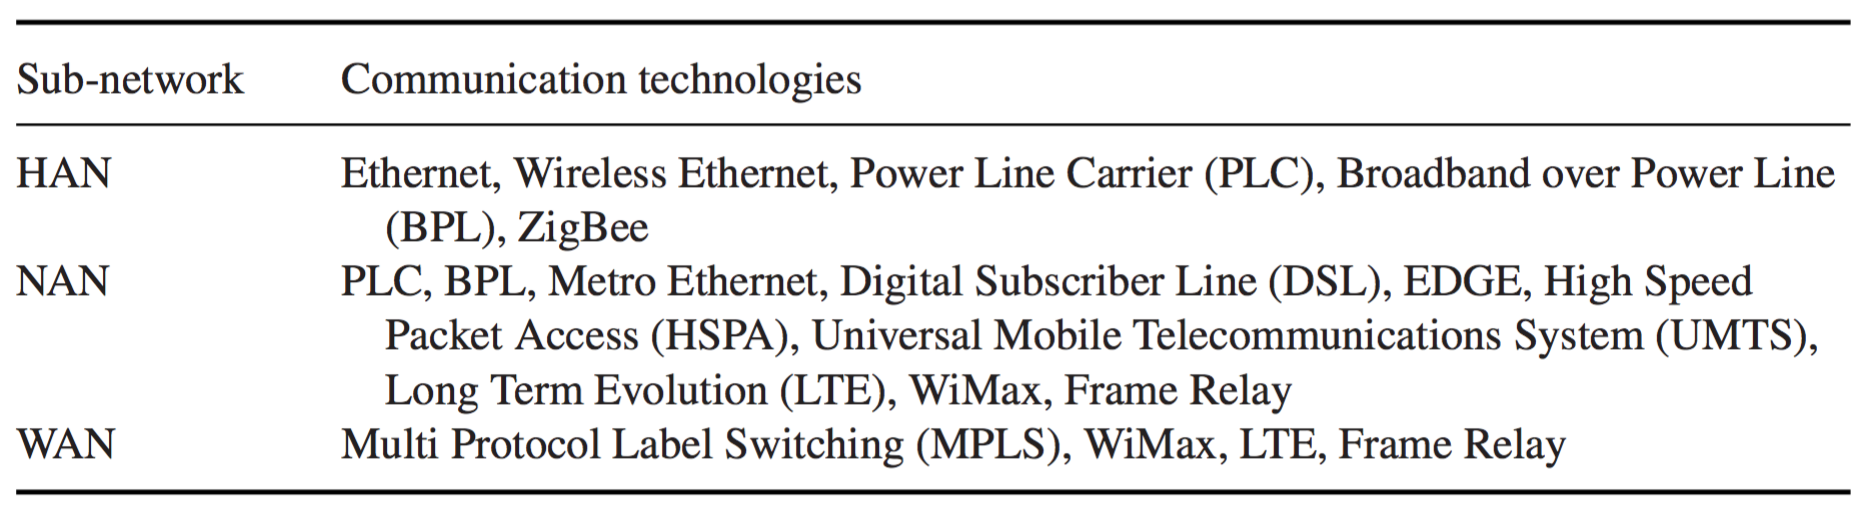
\includegraphics[scale=0.350]{imgs/tech.png}
	\caption{Tecnologie usate nelle differenti sottoreti} \label{fig:th}
\end{figure}

\section{Tecnologie di comunicazione}
\subsection{IEEE 802}
IEEE 802 è una famiglia di standard sviluppati per il supporto alle reti locali (LAN). Facendo riferimento alla Smart Grid, tali standard sono applicabili alle reti LAN in sistemi SCADA, NAN per le reti di distribuzione e HAN nei locali dei clienti.\\
La Figura \ref{fig:arch_802} mostra come l'architettura IEEE 802 è incentrata sui due livelli inferiori del modello ISO/OSI.
\begin{figure}[h]
	\centering
	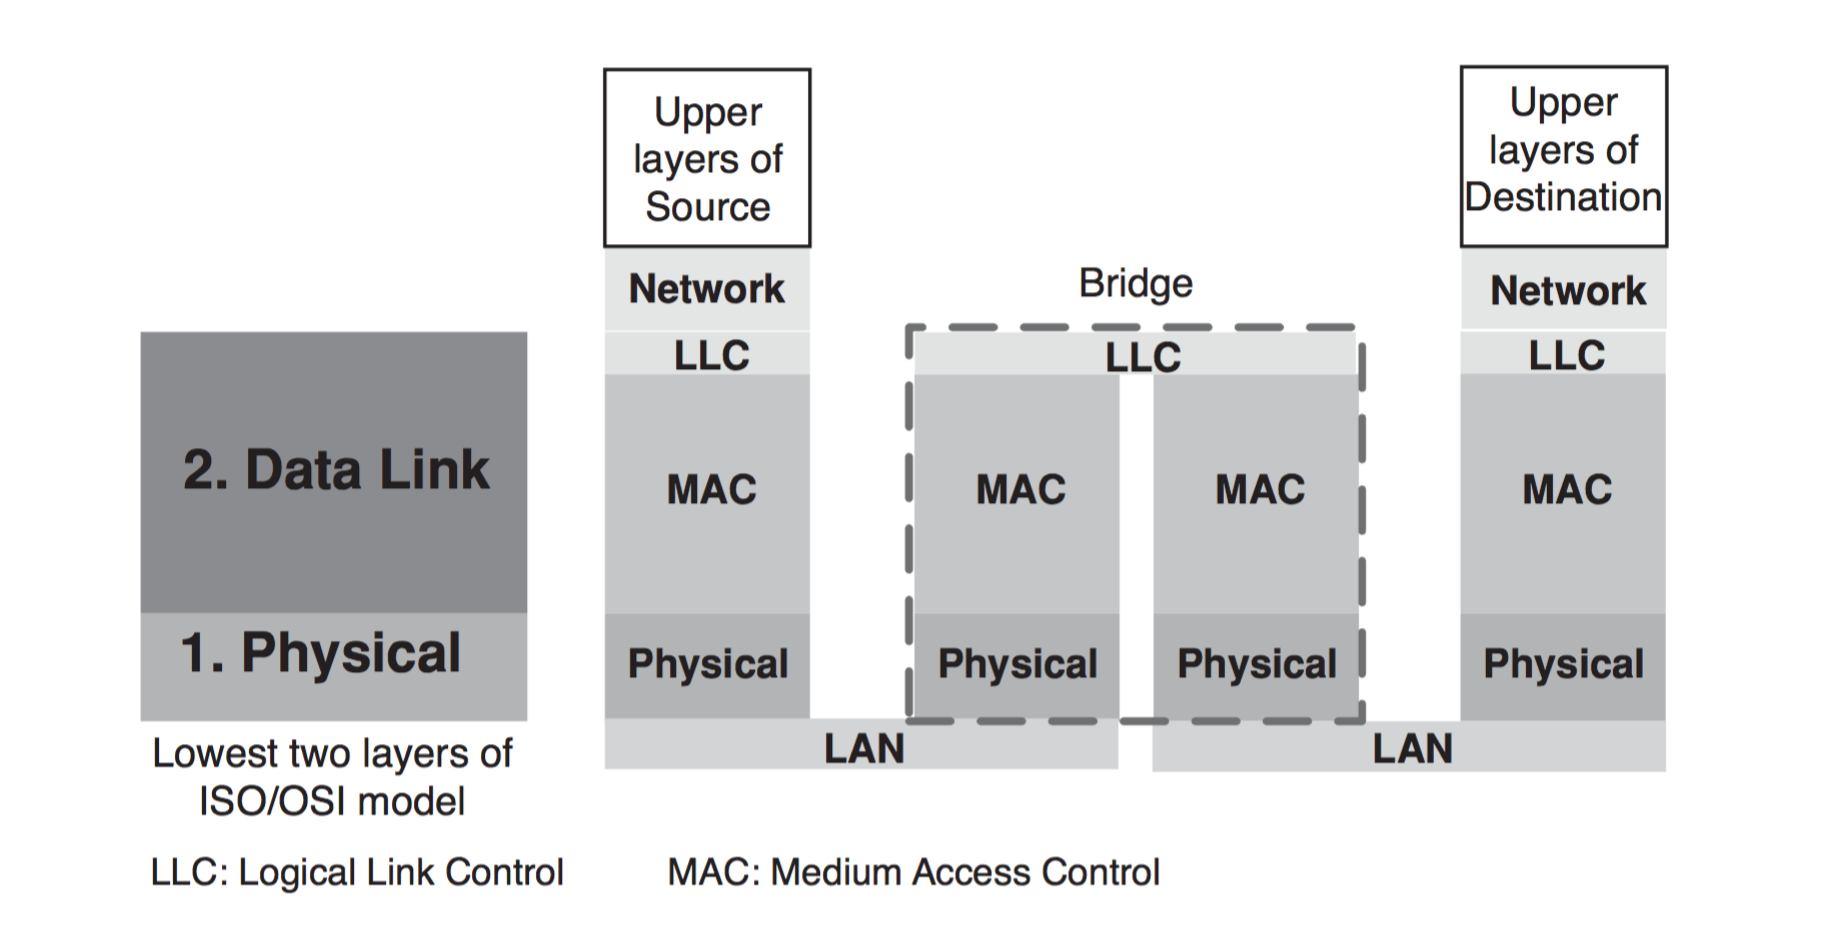
\includegraphics[scale=0.320]{imgs/arch_ieee802.png}
	\caption{Architettura IEEE 802} \label{fig:arch_802}
\end{figure}
\\
In figura è mostrato come due LAN possono essere collegate tramite un Bridge. Tale connessione è comune in molte organizzazioni che hanno più LAN. Un pacchetto dalla sorgente entra nel sottostrato Logical Link Control (LLC) che funge da interfaccia tra il livello di rete e il sottostrato MAC. LLC è definito da IEEE 802.2 e fornisce i meccanismi di controllo del flusso, multiplexing e di controllo degli errori. Il pacchetto passa poi nel sottostrato MAC in cui vengono aggiunti un header e un trailer al pacchetto (a seconda della LAN cui il pacchetto entra). Poi si passa attraverso il livello fisico e il canale di comunicazione e si raggiunge il bridge. A livello MAC del bridge, l'intestazione e il trailer sono rimossi e viene recuperato il pacchetto originale che passa al sottostrato LLC del bridge. Successivamente il pacchetto viene elaborato dal livello MAC (aggiungendo un'intestazione appropriata e un trailer) in base alla LAN a cui si trasmette. L'utilizzo del bridge è essenziale in quanto LAN diverse utilizzano differenze dimensioni del frame e velocità.
%Ad esempio, IEEE 802.3 utilizza un frame di 1500 byte, mentre IEEE 802.4 ne utilizza uno di 8191 byte.
\subsubsection{Ethernet}
Ethernet è diventata la tecnologia di rete più utilizzata per le LAN cablate grazie alla sua semplicità, affidabilità, facilità di manutenzione e la capacità di integrare nuove tecnologie. Essa ha un basso costo di installazione ed è facile da aggiornare. Si tratta di una tecnologia di comunicazione frame-based che si basa sullo standard IEEE 802.3. 
%\\{\color{blue} ?!?Dispositivi ETHERNET?!?}\\
Ethernet utilizza un mezzo condiviso in cui più di un device proverà ad accedervi. Questo causa collisioni tra frame trasmessi dai vari host. Il problema delle collisioni è gestito da un protocollo chiamato Carrier Sense Multiple Access/Collision Detect (CSMA/CD). Un set di host connessi ad una rete in modo tale che la trasmissione simultanea da due host nel set porta a collisioni, crea un \emph{dominio di collisione}. Inoltre, le LAN Ethernet trasportano anche frame di broadcast il cui dominio raggiungibile è denominato \emph{dominio di broadcast}. Le prestazioni della rete, in caso di traffico, sono influenzate dal modo in cui i domini di collisione e di broadcast sono situati e quindi l'idea è quella di isolarli per aumentare le prestazioni della rete.\newpage
La Figura \ref{fig:lan} mostra tali domini su una tipica LAN Ethernet.
\begin{figure}[h]
	\centering
	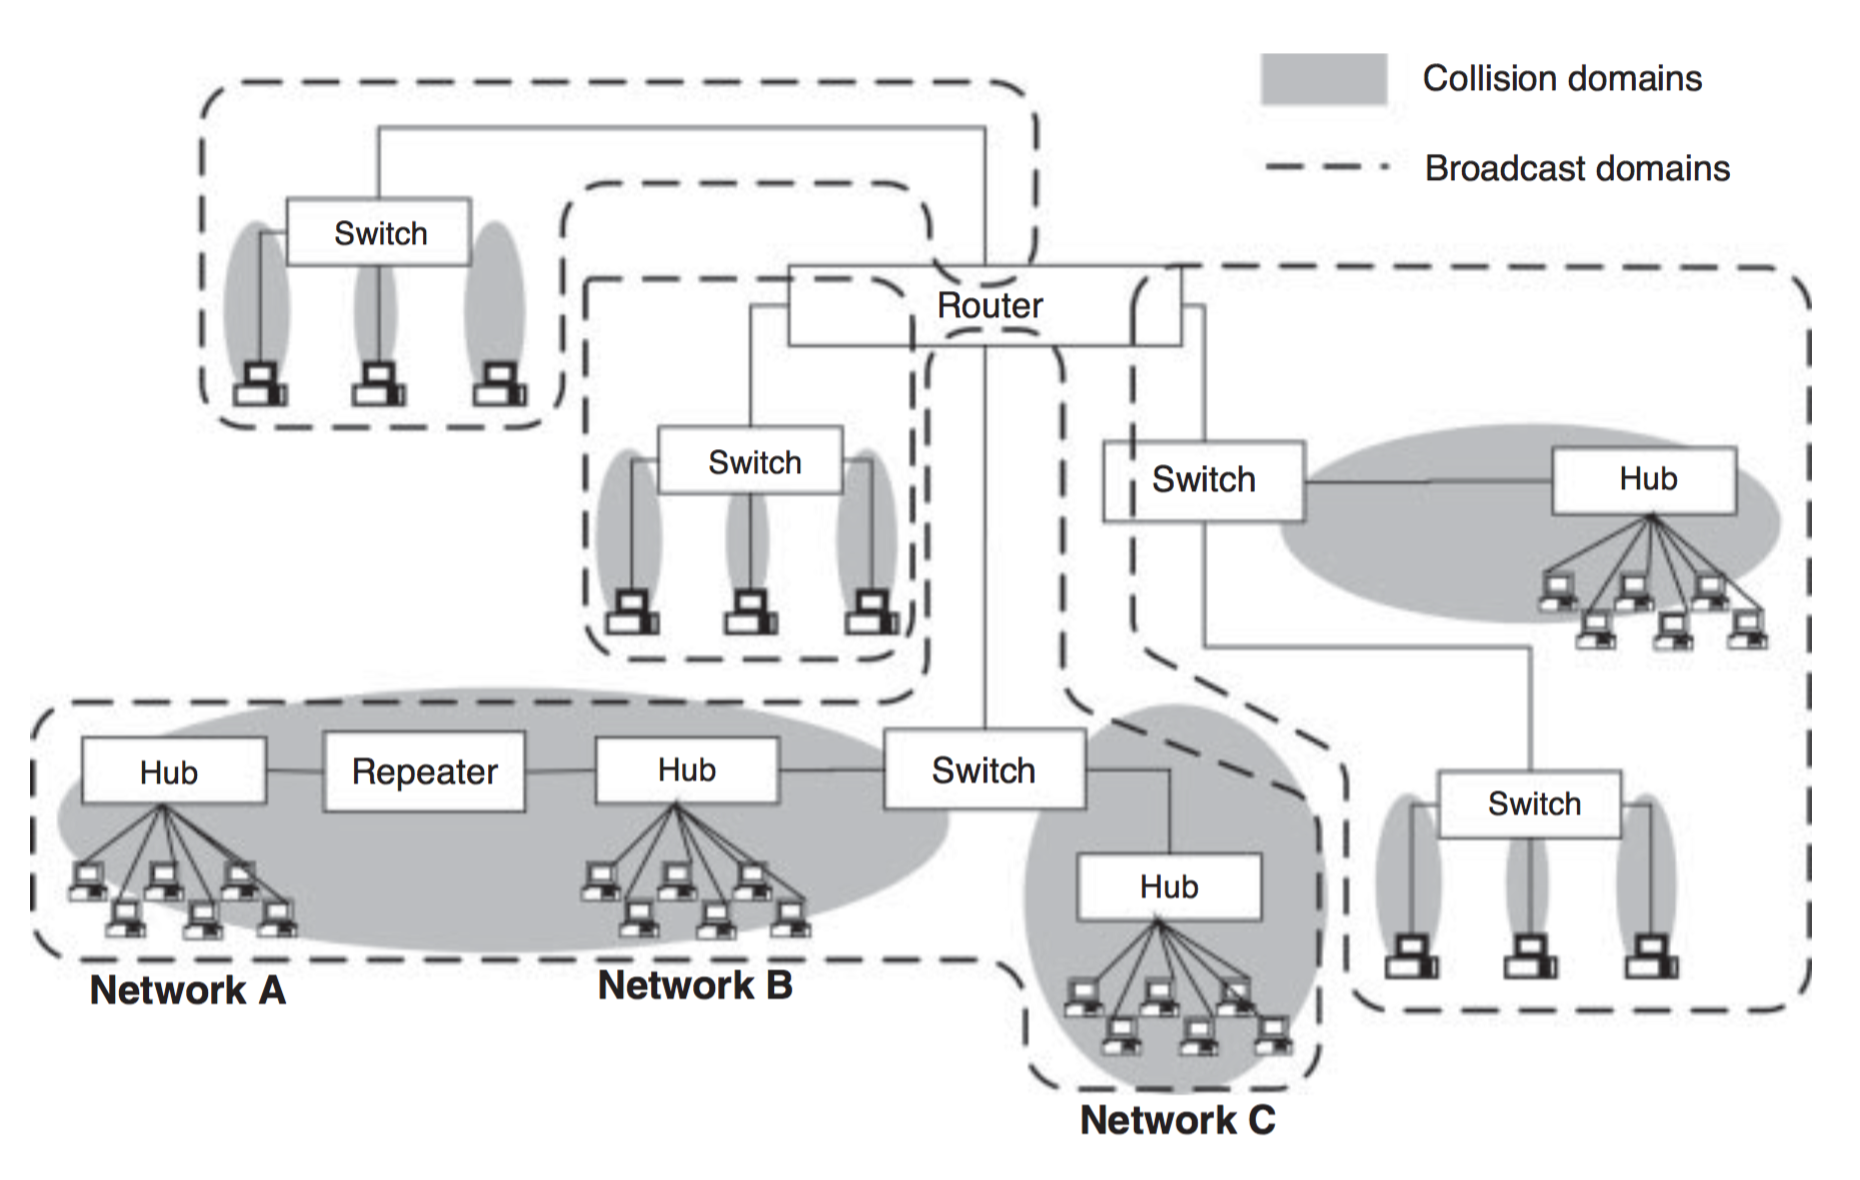
\includegraphics[scale=0.340]{imgs/lan.png}
	\caption{LAN Ethernet} \label{fig:lan}
\end{figure}
\\I Bridge limitano i domini di collisione mentre i Router limitano entrambi i domini. In Figura \ref{fig:lan} è mostrato come un pacchetto inviato dalla rete A può collidere con uno della rete B, ma non con uno inviato da C. Questo accade perchè vi è uno switch che limita i domini di collisione.
\subsubsection{Wireless}%LAN
IEEE 802.11 definisce un insieme di standard per le Wireless LAN (WLAN). L'interoperabilità dei dispositivi IEEE 802.11 è certificata dalla Wi-Fi Alliance. Una LAN Wireless è costituita dai seguenti componenti:
\begin{itemize}
	\item\emph{Station}: descrive qualsiasi dispositivo che comunica tramite una rete WLAN, ad esempio, un computer portatile, o cellulari che supportano WiFi. Nelle reti ad-hoc questi dispositivi possono comunicare tra loro, creando una rete mesh (vedi Figura \ref{fig:bss}a). L'insieme di station che formano la rete ad-hoc è chiamato Independent Basic Service Set (IBSS);
	\item\emph{Access Point (AP)}: consente ad una stazione di comunicare con un altra facendo da tramite. Necessita il doppio della larghezza di banda necessaria se la stessa comunicazione avvenisse direttamente tra le stazioni comunicanti. Gli AP rendono il sistema scalabile e consentono la connessione cablata con altre reti. In presenza di AP (vedi Figura \ref{fig:bss}b) l'insieme delle station è chiamato Infrastructure BSS;
	\item\emph{Distribution System}: interconnette Infrastructure BSS attraverso gli AP, come mostrato nella Figura \ref{fig:ds}. Facilita la comunicazione tra gli AP, l'inoltro del traffico da un BSS ad un altro ed il movimento di mobile station tra BSS. Un insieme di Infrastructure BSS è chiamato Extended Service Set (ESS).
\end{itemize}
La famiglia di reti LAN Wireless 802.11 utilizza il protocollo CSMA/CA per l'accesso al mezzo trasmissivo. Sono noti vari standard identificati da 802.11a/b/g/n/ac con variazioni a livello fisico. Una tipica applicazione di 802.11 nelle Smart Grid è mostrata in Figura \ref{fig:802_sg}.
\begin{figure}[h]
	\centering
	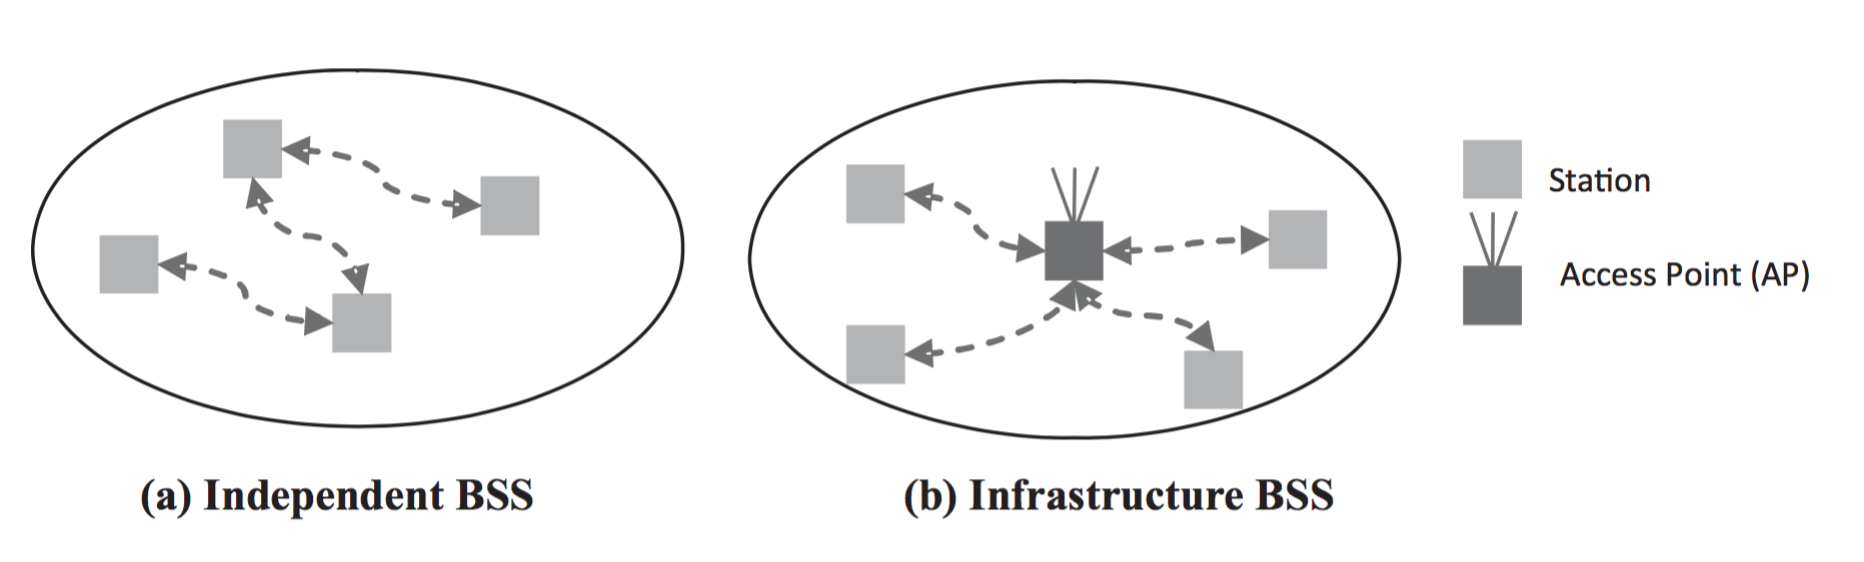
\includegraphics[scale=0.350]{imgs/bss.png}
	\caption{Architetture BSS di WLAN} \label{fig:bss}
\end{figure}
\begin{figure}[h]
	\centering
	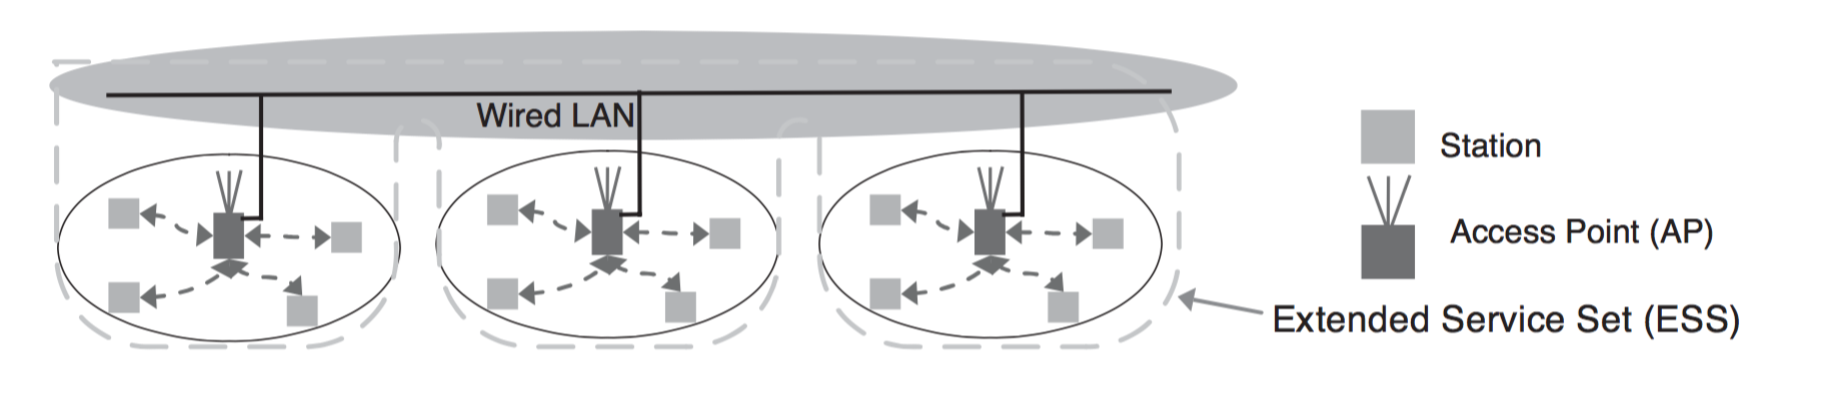
\includegraphics[scale=0.350]{imgs/ds.png}
	\caption{Distribution System} \label{fig:ds}
\end{figure}
\begin{figure}[h]
	\centering
	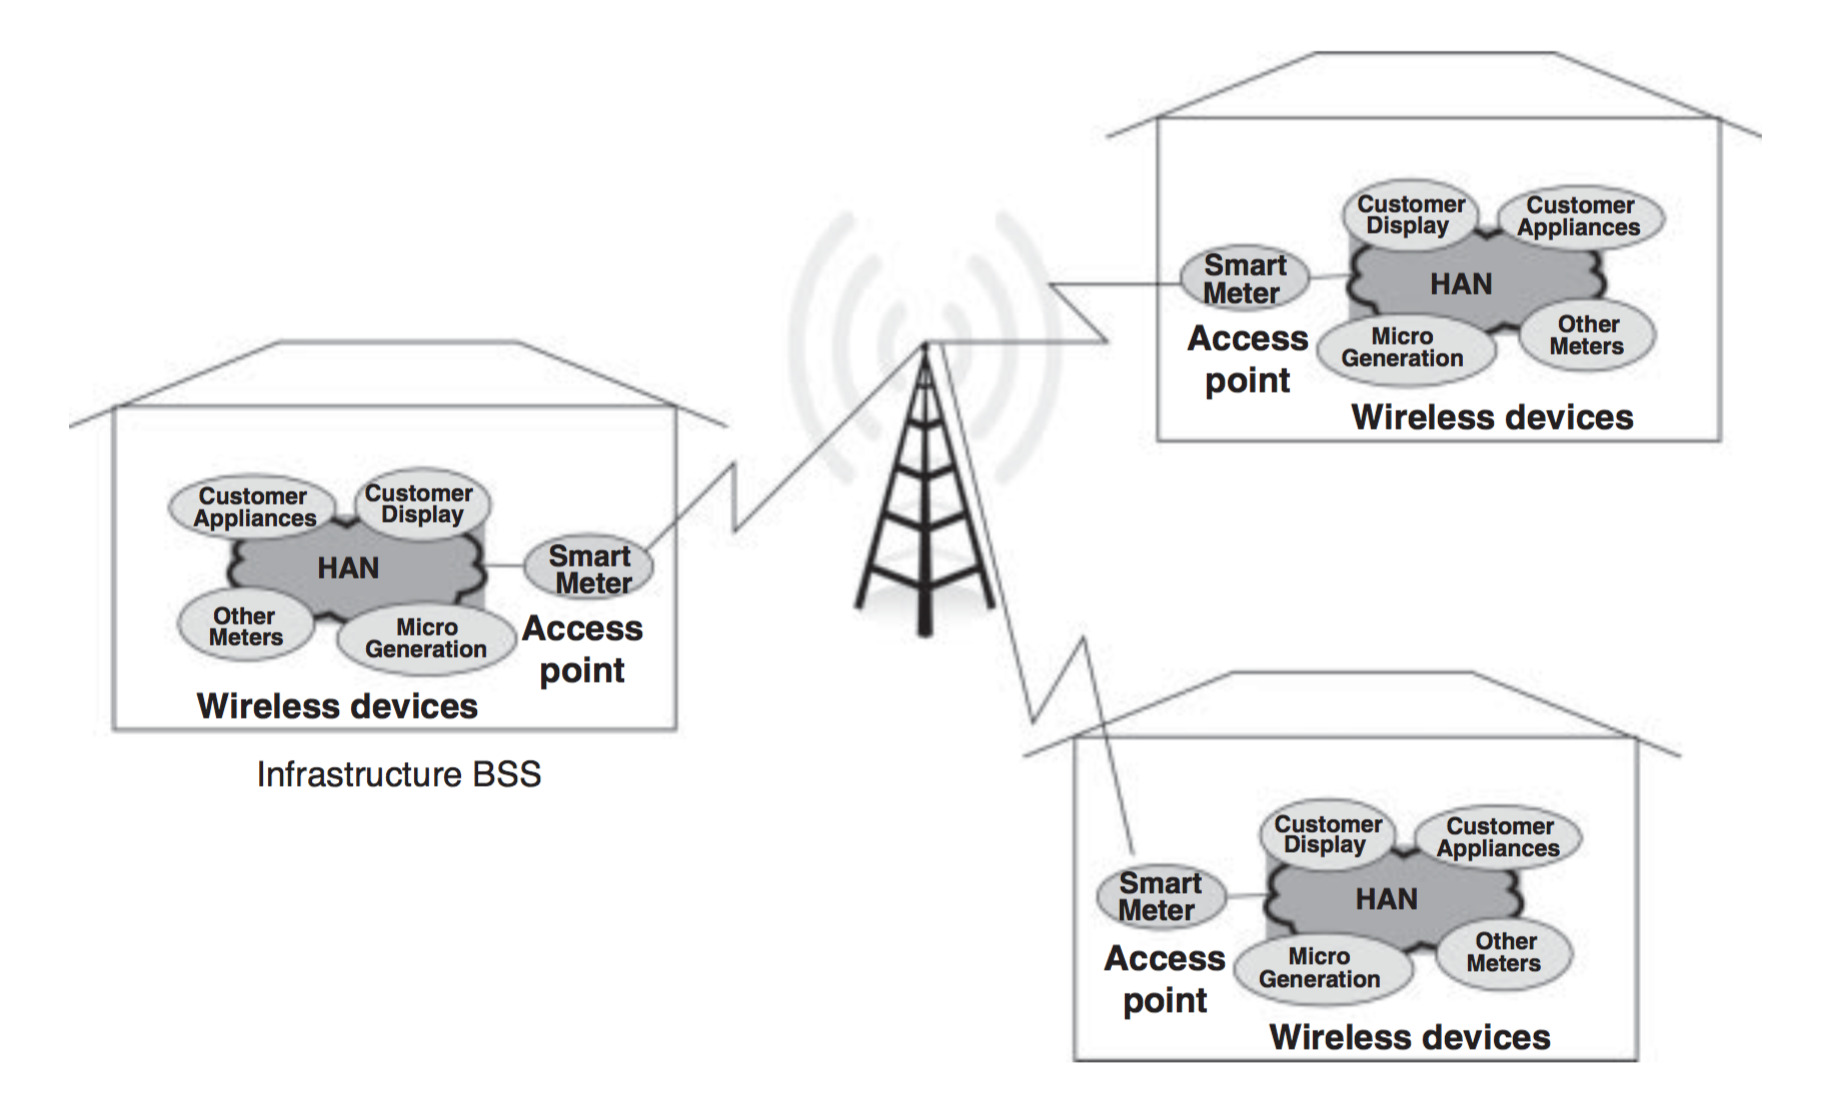
\includegraphics[scale=0.350]{imgs/80211smartgrid.png}
	\caption{Applicazione di WLAN 802.11 in una Smart Grid} \label{fig:802_sg}
\end{figure}\newpage
\subsubsection{Bluetooth}
Bluetooth, definito dallo standard IEEE 802.15.1, è una tecnologia LAN wireless progettata per collegare i dispositivi mobili o fissi con bassi consumi, un corto raggio d'azione (fino a 100 metri di copertura per un dispositivo di Classe 1 e fino ad un metro per dispositivi di Classe 3) e un basso costo di produzione per i dispositivi compatibili. 
%{\color{blue} ?!?VERSIONI?!?}\\
Bluetooth definisce due architetture di rete denominate Piconet e Scatternet. La Piconet è costituita da un dispositivo \emph{Master} e fino a sette dispositivi \emph{Slave}. Altri dispositivi possono sincronizzarsi col Master ma non possono partecipare alla comunicazione. Si dice che tali dispositivi sono in un parked state. Un device in parked state può passare in active state se il numero di Slave della Piconet è inferiore a sette. Le Piconet possono essere interconnesse attraverso un Bridge che può essere Slave per una Piconet e Master per un'altra oppure Slave per due Piconet che sono interconnesse come in Figura \ref{fig:bt}a e \ref{fig:bt}b. Un insieme di Piconet forma una Scatternet.\newline
Possono essere creati due tipi di collegamenti bluetooth per il trasferimento dei dati:
\begin{itemize}
		\item Synchronous Connection Orientated (SCO) link
		\item Asynchronous Connectionless Link (ACL)
\end{itemize}
SCO è utilizzato quando la consegna tempestiva è più importante della consegna senza errori mentre ACL è utilizzato nel caso opposto.
\\
\begin{figure}[h]
	\centering
	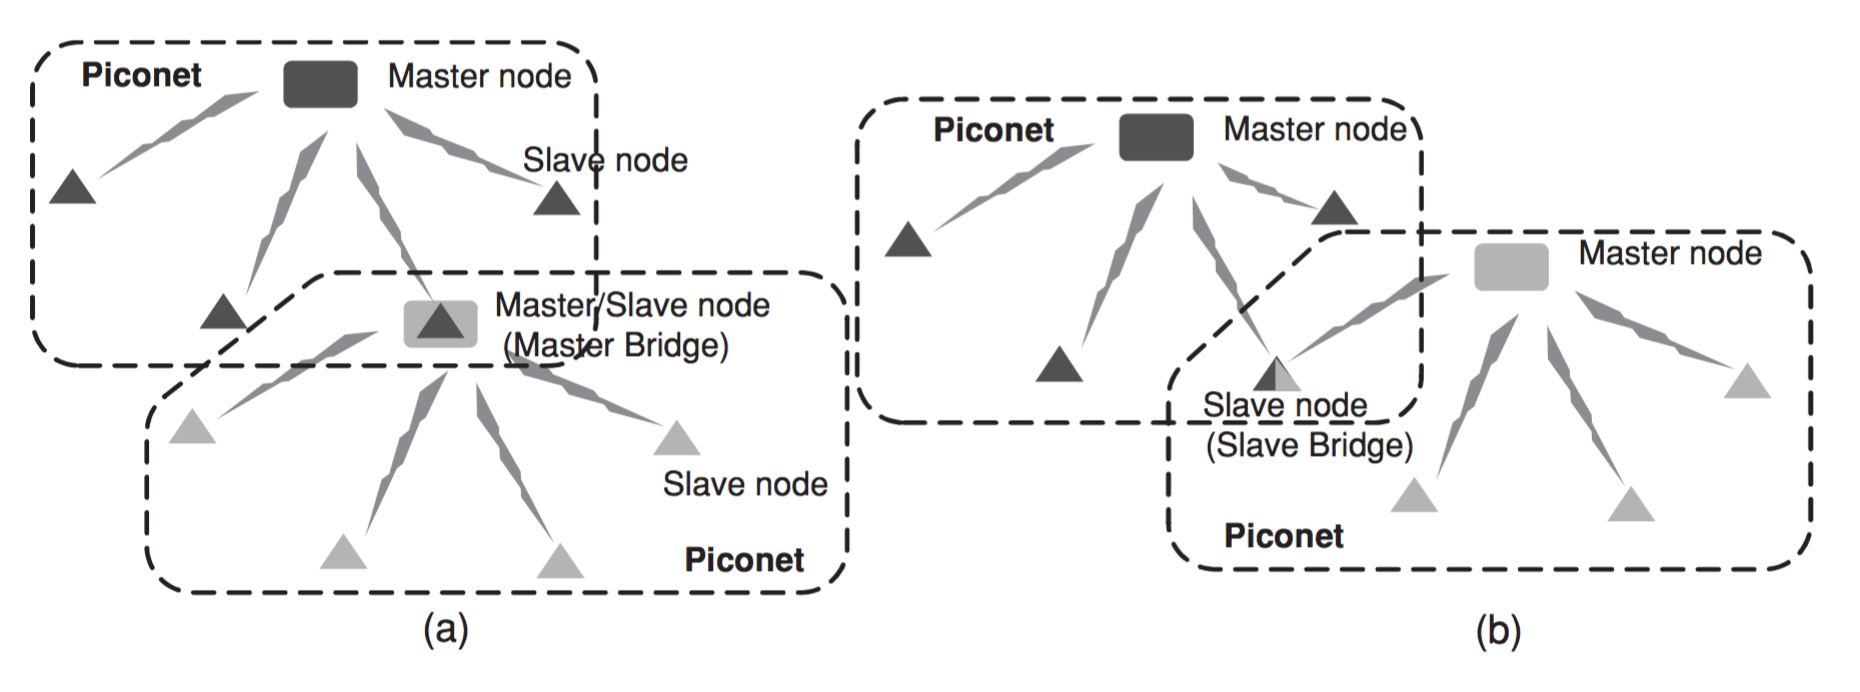
\includegraphics[scale=0.350]{imgs/bt.png}
	\caption{Piconet e Scatternet} \label{fig:bt}
\end{figure}
\subsubsection{ZigBee and 6LoWPAN}
ZigBee e 6LoWPAN sono due tecnologie di comunicazione basate su IEEE 802.15.4 per Wireless Personal Area Network (WPAN) dato il basso consumo, l'alta flessibilità ed il basso costo. L'architettura protocollare di un device ZigBee è mostrata nella Figura \ref{fig:zbprot} in cui i due strati inferiori sono definiti da IEEE 802.15.4. Application Support e Network Layer per la rete ZigBee sono definiti dalla ZigBee Alliance\cite{zb}.
\begin{figure}[h]
	\centering
	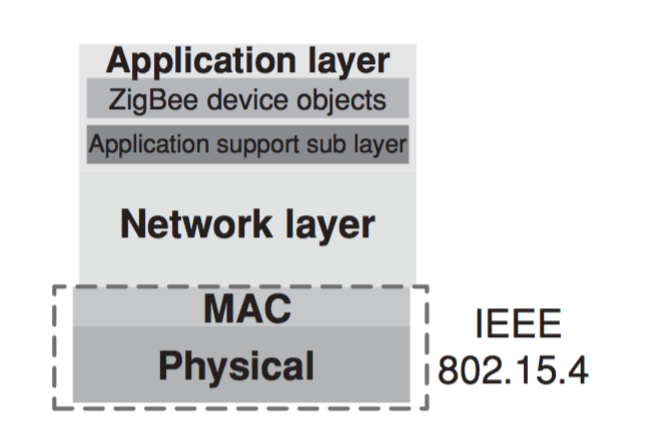
\includegraphics[scale=0.350]{imgs/zbprot.png}
	\caption{Architettura Protocollare di ZigBee} \label{fig:zbprot}
\end{figure}
Un device ZigBee può essere un Full Function Device (FFD) o un Reduced Function Device (RFD). Una rete avrà almeno un FFD, che fungerà da coordinatore della WPAN. Il FFD può funzionare in tre modalità: coordinatore, router o device. Un RFD può funzionare solo come device. Un FFD può interagire sia con un altro FFD che con un RFD, mentre un RFD può parlare solo con un FFD.
La tecnologia ZigBee è quindi considerata come una buona opzione per il metering e la gestione dell'energia ideale in implementazioni Smart Grid data la semplicità, mobilità, robustezza e i bassi costi di sviluppo. Offre anche programmi di pricing e monitoraggio del sistema real-time. ZigBee presenta però alcuni vincoli relativi alle basse capacità di elaborazione, alla piccola dimensione della memoria e alle interferenze tra i vari apparecchi che condividono lo stesso mezzo trasmissivo. Tali problematiche in condizioni di rumore aumentano la possibilità di danneggiare il canale di comunicazione a causa delle interferenze. Schemi di interference detection/avoidance e protocolli di routing energy-efficient estendono il tempo di vita della rete e forniscono una performance di rete affidabile e ad alta efficienza energetica.
\newline\newline
6LoWPAN è un protocollo che consente l'invio e la ricezione di pacchetti IPv6 nelle reti basate su IEEE 802.15.4. In tale protocollo è stato inserito un Adaptation Layer (vedi Figura \ref{fig:6pan}) per il collegamento tra lo strato MAC e il Network Layer IPv6.
%Il concetto 6LoWPAN nasce dall'idea che "il protocollo Internet potrebbe e dovrebbe essere applicato anche ai dispositivi più piccoli," e che i dispositivi a bassa potenza e con capacità di elaborazione limitate dovrebbero essere in grado di far parte dell' Internet of Things.
\begin{figure}[h]
	\centering
	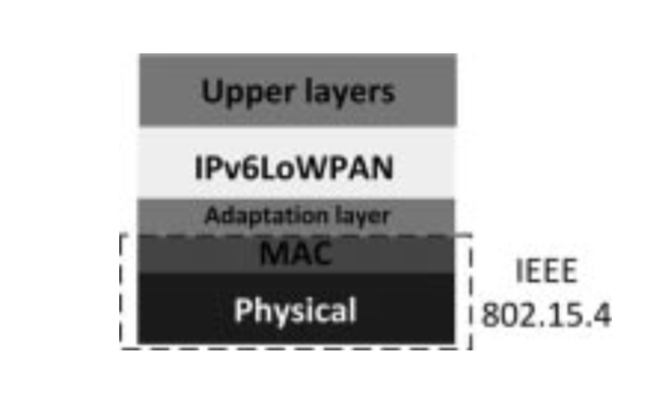
\includegraphics[scale=0.350]{imgs/6pan.png}
	\caption{Architettura Protocollare di ZigBee} \label{fig:6pan}
\end{figure}
\\
Quando un RFD in un 6LoWPAN vuole inviare un pacchetto di dati ad un dispositivo che si trova al di fuori del dominio 6LoWPAN, invia il pacchetto a un FFD nella stessa WPAN. Il FFD che agisce da router nella 6LoWPAN inoltrerà il pacchetto dati di hop in hop fino al gateway 6LoWPAN. Il gateway 6LoWPAN potrà quindi inoltrare il pacchetto al dispositivo di destinazione utilizzando l'indirizzo IP (vedi Figura \ref{fig:6pancom}).
\begin{figure}[h]
	\centering
	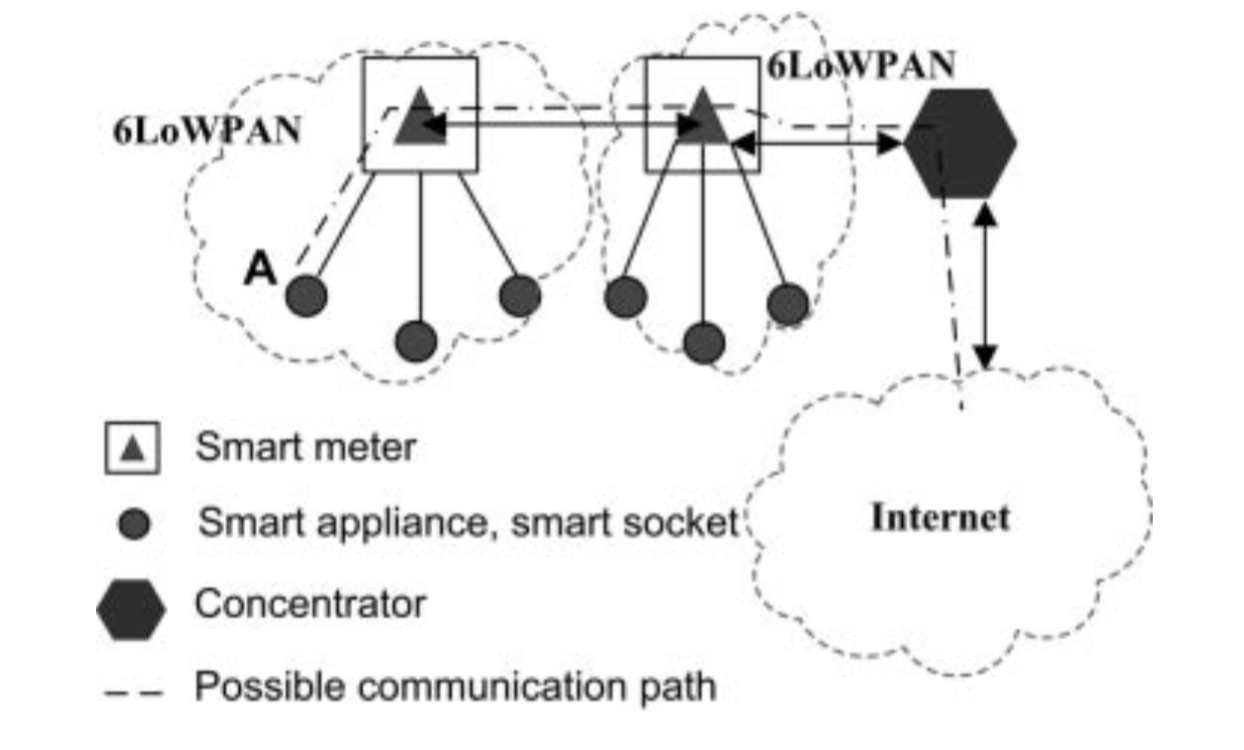
\includegraphics[scale=0.350]{imgs/6pancom.png}
	\caption{Comunicazione in una rete 6LoWPAN} \label{fig:6pancom}
\end{figure}
\subsubsection{WiMax}
Worldwide Interoperability for Microwave Access (WiMAX) è una tecnologia wireless conforme allo standard IEEE 802.16. Fornisce sia connettività fissa che mobile usando una tecnica chiamata Orthogonal Frequency Division Multiple Access (OFDMA). La rete WiMax è mostrata in Figura \ref{fig:wim}. La copertura del WiMax si estende fino a 50 km con una velocità di trasferimento dati di picco di 75 Mbps per i collegamenti fissi e fino a 15 Mbps per connessioni mobili. È ottimizzato per supportare dispositivi mobili fino ad una velocità di 10 km/h. Anche se supporta veicoli in movimento fino a 120 km/h, le sue prestazioni degradano con l'aumentare della velocità del veicolo.
\begin{figure}[h]
	\centering
	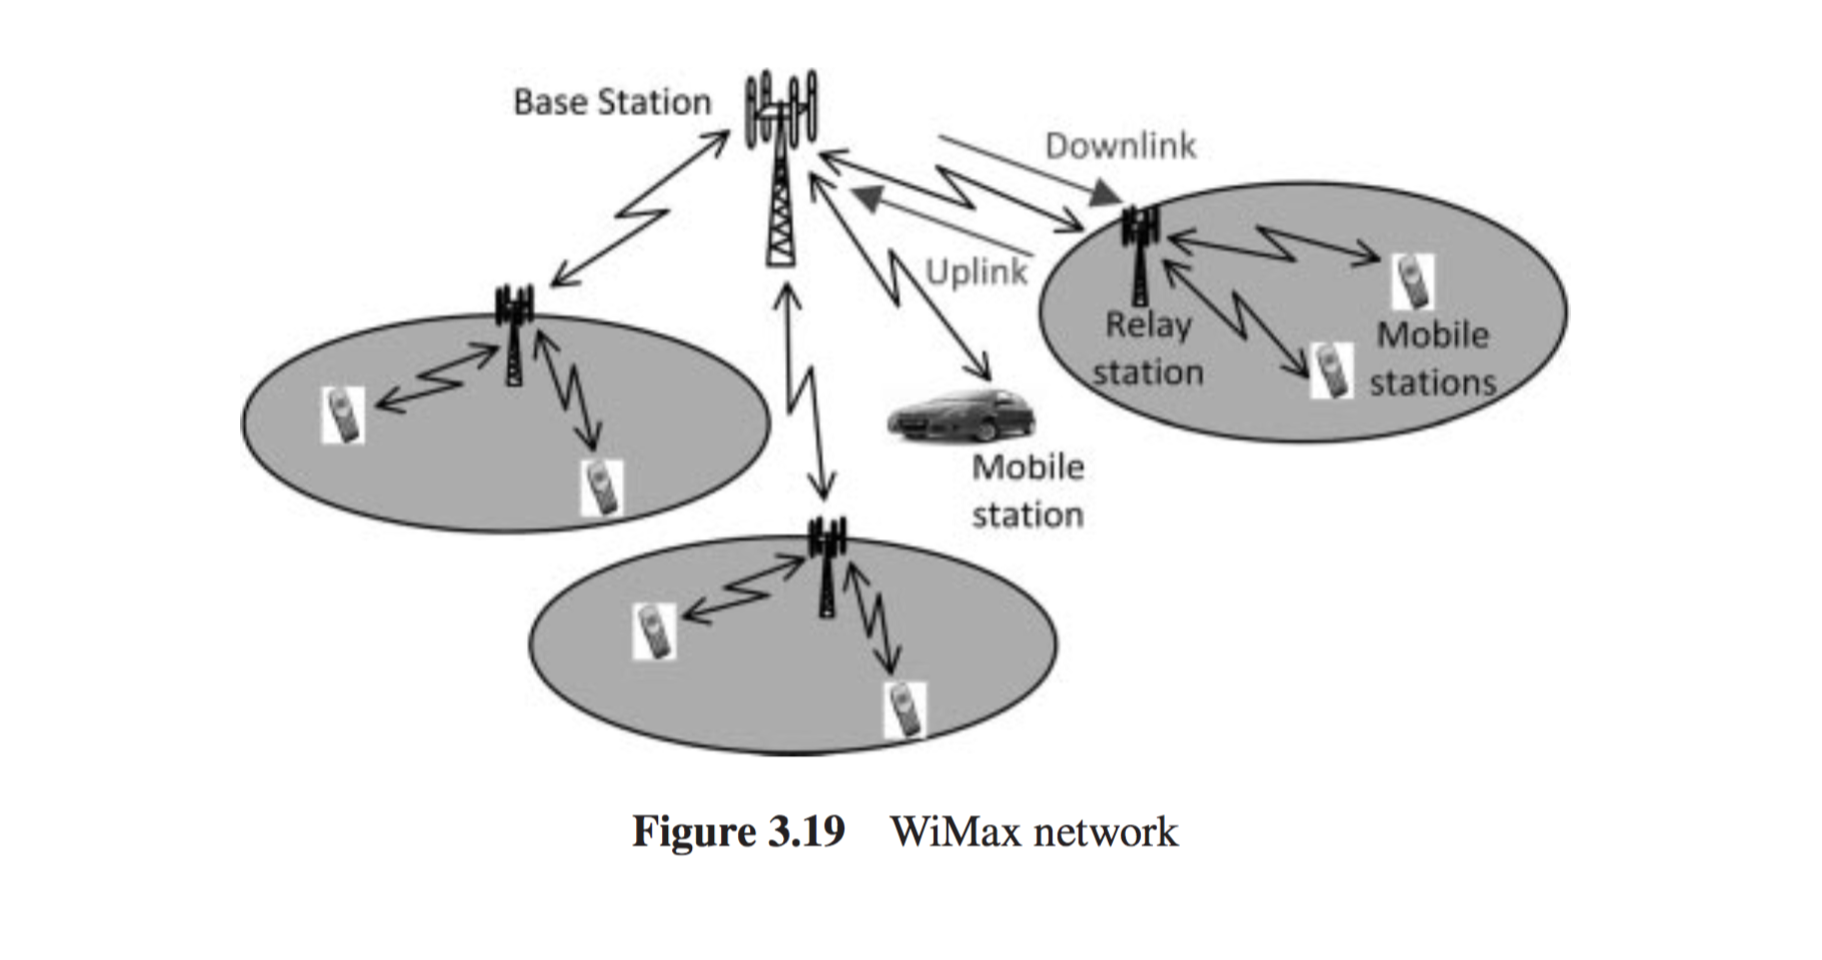
\includegraphics[scale=0.350]{imgs/wim.png}
	\caption{Una rete WiMax} \label{fig:wim}
\end{figure}
\subsection{Power line}
La Power Line Communication (PLC) rappresenta una delle tecnologie di rete proposte per la trasmissione in ambiente Smart Grid in quanto l'infrastruttura esistente riduce i costi di installazione di un'ulteriore infrastruttura di comunicazione. PLC trasporta i dati utilizzando un conduttore e le linee elettriche esistenti. Fornisce servizi di comunicazione per Automatic Meter Reading (AMR), AMI e HAN ma anche l'accesso ad internet all'utente finale. In una tipica rete PLC, gli smart meter sono collegati al data concentrator attraverso power line e i dati vengono trasferiti al data center tramite tecnologie di rete cellulare. La tecnologia PLC è infatti scelta per la comunicazione tra gli smart meter e il data concentrator, mentre la tecnologia GPRS è utilizzata per trasferire i dati dal concentrator al data center. Anche l'ENEL, nota azienda multinazionale produttrice e distributrice di energia elettrica, ha scelto la tecnologia PLC per trasferire i dati degli smart meter al data concentrator più vicino e la tecnologia GSM per inviare i dati al data center. 
%data concentrator = dispositivo che collezionana informazioni e dati, spesso da più meter, prima di fare il forwarding al data center. Spesso utilizzato in aree dense.
La topologia di rete, il numero e il tipo dei dispositivi collegati, la distanza tra trasmettitore e ricevitore compromettono la qualità del segnale. La sensibilità di PLC ai disturbi e la dipendenza sulla qualità segnale sono gli svantaggi che rendono la tecnologia non adatta alla trasmissione dei dati. Tuttavia, ci sono state alcune soluzioni ibride in cui la tecnologia PLC si combina con altre, ad esempio, GPRS o GSM, per fornire una connettività non possibile dalla tecnologia PLC. Inizialmente la velocità di trasmissione in questo tipo di reti era molto limitata, fino a pochi kbps. Successivamente, grazie al progresso tecnologico, con l'introduzione di broadband PLC (BB-PLC) la velocità di trasmissione ha raggiunto anche i 200 Mbps. Principalmente sono utilizzate tre diverse tecnologie di comunicazione, vale a dire, \emph{narrowband transmission}, \emph{spread-spectrum transmission} e \emph{DSP-processed narrowband transmission}. La Figura \ref{fig:vs_plc} mostra alcuni vantaggi e svantaggi relativi a PLC in ambito Smart Grid.
\begin{figure}[h]
	\centering
	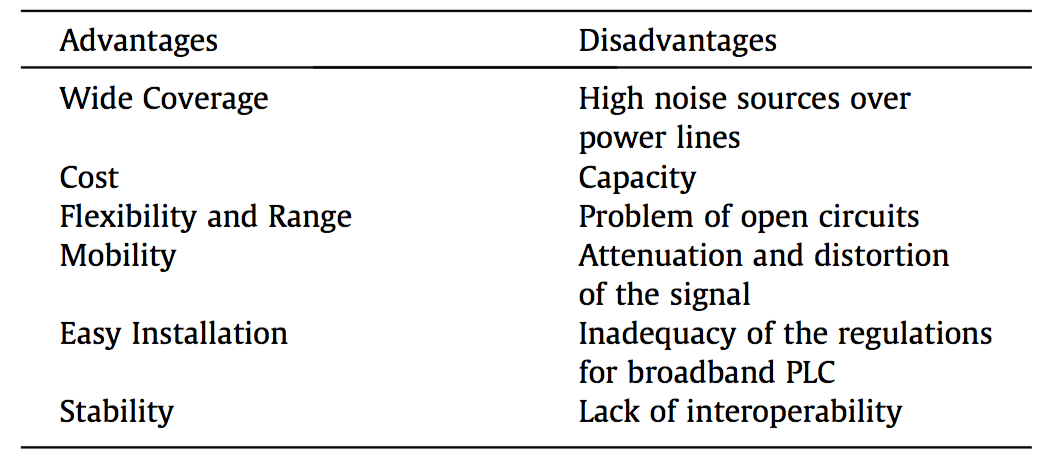
\includegraphics[scale=0.350]{imgs/vs_plc.png}
	\caption{Vantaggi e Svantaggi di PLC in ambito Smart Grid} \label{fig:vs_plc}
\end{figure}\\
Tra gli standard e i protocolli maggiormente utilizzati troviamo IEEE P1901 e HomePlug.
\newpage
\subsubsection{IEEE P1901}
Il gruppo IEEE P1901 è stato formato nel 2005 con lo scopo di sviluppare una tecnologia per la trasmissione di voce o dati che utilizzi la rete di alimentazione elettrica come mezzo trasmissivo. Lo standard permette una comunicazione ad altà velocità tra i device che prendono il nome di BPL (Broadband over Power Line). Lo standard utilizza frequenze inferiori a 100 MHz ed è di supporto ai device BPL utilizzati per i collegamenti first-mile/last-mile così come quelli utilizzati nelle reti LAN all'interno di edifici. Inoltre tali device possono essere utilizzati all'interno di smart energy application, autoveicoli e in altre applicazioni per la distribuzione dei dati.
\subsubsection{HomePlug}
HomePlug è una tecnologia broadband non standardizzata e specificata dalla HomePlug Powerline Alliance, i cui membri sono le principali aziende nel settore della comunicazione e dell'energia. Il protocollo gestisce dei sottocanali dividendo la larghezza di banda disponibile. La velocità di trasmissione varia da 1 a 14 Mbps e i nodi sono in grado di adattarsi al data rate ottimale in maniera automatica. Le collisioni sono evitate grazie al CSMA / CD. Lo standard HomePlug 1.0 per la connessione di dispositivi nelle case (1-10 Mbps) utilizza la di tecnica Orthogonal Frequency Division (OFDM), utilizzata anche da DSL, IEEE 802.11a e IEEE 802.11g. Il rumore, comune in ambiente power line, è superato per mezzo di forward error correction e data interleaving. La HomePlug Powerline Alliance ha definito ulteriori standard come HomePlug AV/AV2 che forniscono banda sufficiente per applicazioni come HDTV e VoIP, HomePlug CC e HomePlug BPL.
\section{Standard per lo scambio di informazioni}
\subsubsection{Standard per Smart Meter}
Gli Smart Meter possono essere utilizzati in vari modi e questi portano a differenti requisiti per quanto riguarda il sistema di comunicazione. Con Automated Meter Reading (AMR) si richiede una trasmissione occasionale dei dati energetici registrati (circa una volta al mese), viceversa con  Advanced Metering Infrastructure (AMI) si richiedono frequenti comunicazioni bidirezionali (ad esempio ogni 30 minuti). IEC 62056 e ANSI C12.22 sono due famiglie di standard che descrivono sistemi di comunicazione per gli Smart Meter. IEC 62056 definisce Transport e Application Layer per lo smart metering nell'ambito di una serie di specifiche chiamate COSEM (Companion Specification for Energy Metering). ANSI C12.22 (vedi Figura \ref{fig:arch_c1222}) specifica l'invio e la ricezione dei dati registrati da e verso sistemi esterni ed è possibile utilizzarlo su qualsiasi rete di comunicazione.
\begin{figure}[h]
	\centering
	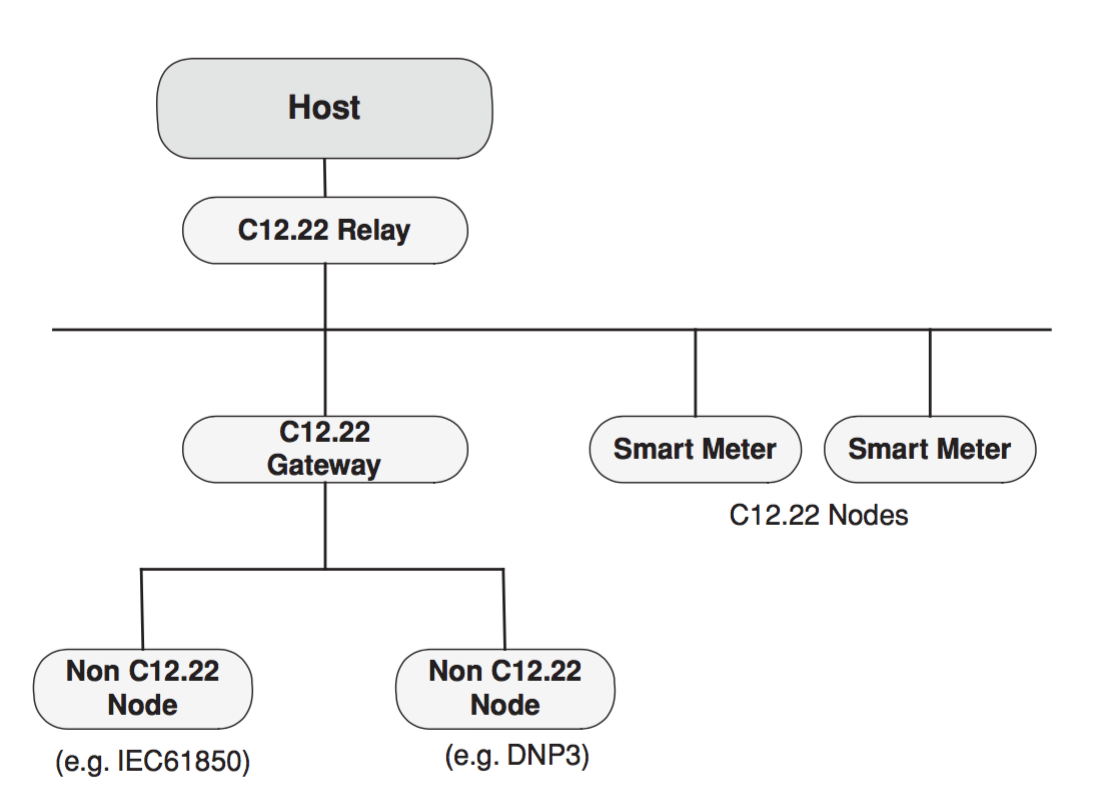
\includegraphics[scale=0.350]{imgs/arch_c1222.png}
	\caption{Architettura ANSI C12.22} \label{fig:arch_c1222}
\end{figure}
\newpage
\subsubsection{Modbus}
Modbus è un protocollo di messaggistica che risiede nello strato delle applicazioni e consente la comunicazione tra i dispositivi collegati su diversi bus e reti. Può essere implementato tramite Ethernet o utilizzando la trasmissione seriale asincrona su EIA 232, EIA 422, EIA 485 e fibra ottica. Di questi, l'applicazione più comune è Modbus su EIA485. La Figura \ref{fig:modbus} mostra come l'Application Layer è connesso agli altri layer del modello OSI.
Modbus su EIA 485 è ampiamente usato nell' automazione delle sottostazioni. La comunicazione è avviata dal Master con una query. Il Master è l'unico che può inviare query che possono essere destinate al singolo Slave o di broadcast. Uno Slave monitora continuamente la rete riconoscendo solo le query destinate ad esso.  All'arrivo di una query, lo Slave eseguirà un'azione o risponderà.
\begin{figure}[h]
	\centering
	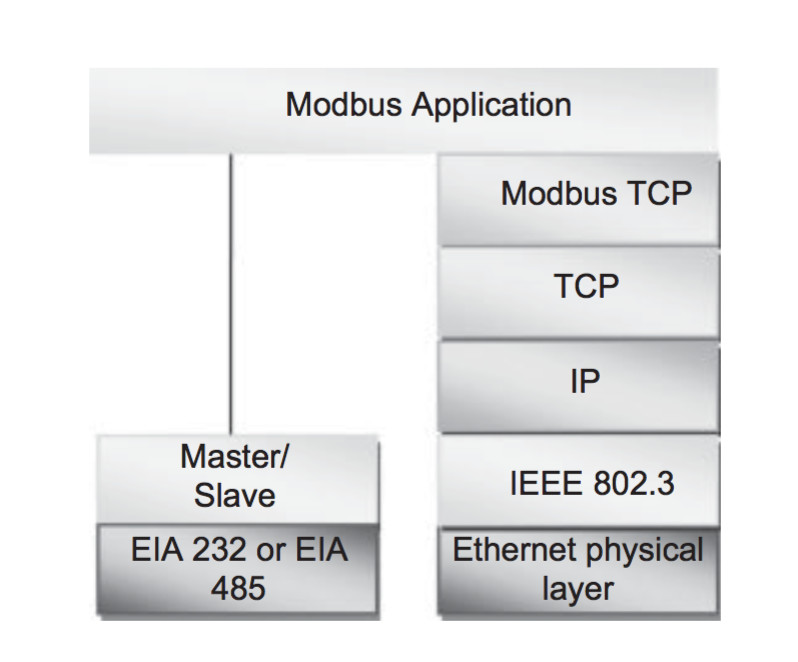
\includegraphics[scale=0.350]{imgs/modbus.png}
	\caption{Modbus stack} \label{fig:modbus}
\end{figure}
\subsubsection{DNP3}
DNP3 è un insieme di protocolli di comunicazione utilizzato tra i componenti nei sistemi di automazione. DNP3 gioca un ruolo fondamentale all'interno dei sistemi SCADA dove è utilizzato dalle SCADA Master Station (conosciute anche col nome di centri di controllo) per comunicare con le Remote Terminal Unit (RTU) e/o gli Intelligent Electronic Device (IED). Lo User Layer DNP ha input analogici e binari e da in output segnali analogici e binari. Un Master DNP3 invia richieste e in genere le stazioni Slave DNP3 rispondono a tali richieste. Uno Slave DNP3 può anche trasmettere un messaggio senza aver ricevuto alcuna richiesta. Il Physical Layer DNP3 utilizza protocolli di comunicazione seriali come EIA 232 o EIA 485. Poiché nelle applicazioni di tipo Smart Grid generalmente si presume l'accesso di terze parti alla stessa rete e all'infrastruttura sottostante basata su protocollo IP, è stato fatto molto lavoro con l'intento di aggiungere caratteristiche di Autenticazione sicura al protocollo DNP3. Alcuni vendors supportano la crittografia via \textbf{bump-in-the-wire} (cioè con dispositivi esterni che criptano/decriptano i dati agli estremi del canale di comunicazione) per le comunicazioni seriali e tramite VPN per le reti IP. Uno dei metodi bump-in-the-wire più popolari era noto come \emph{AGA-12} (American Gas Association).
\subsubsection{IEC 61850}
IEC 61850 è uno standard per la progettazione dei sistemi di automazione per le sottostazioni elettriche. Generalmente questi protocolli girano su reti TCP/IP o LAN di stazione con switch ethernet molto performanti per rispondere ai requisiti stringenti dei dispositivi di protezione, che necessitano tempi di risposta inferiori a 4 o 5 millisecondi. Si tratta di uno standard function-based:
\begin{itemize}
	\item System support functions;
	\item System configuration or maintenance functions;
	\item Operational or control functions;
	\item Process automation functions.
\end{itemize}
IEC 61850 specifica una data structure. Come mostrato in Figura \ref{fig:iec61850}a, un device model considera inizialmente un physical device. Poi vengono specificati i logical device all'interno di tale dispositivo. Ogni logical device è mappato in 86 diverse classi di logical node secondo lo standard IEC 61850. Infine sono specificati i dati relativi a ciascun logical node. Nella Figura \ref{fig:iec61850}b è mostrato un esempio di IED. IEC 61850 è affiancato da IEC 62351 che garantisce la sicurezza e specifica i requisiti tecnici che devono essere rispettati dai fornitori.
\begin{figure}[h]
	\centering
	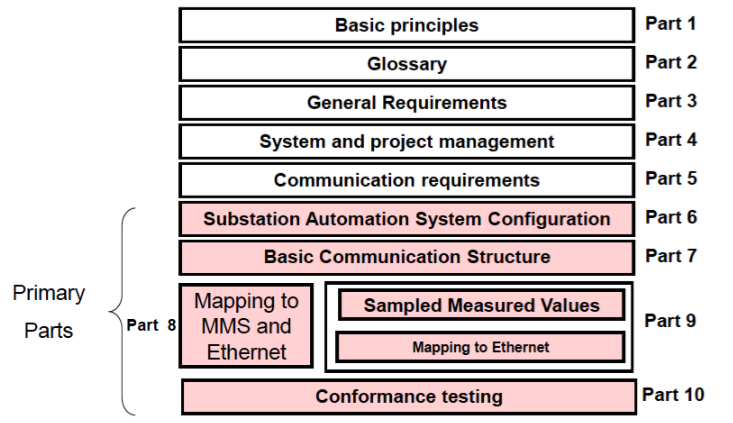
\includegraphics[scale=0.350]{imgs/iec61850.png}
	\caption{IEC 61850 data structure} \label{fig:iec61850}
\end{figure}\\
\section{Standard per la sicurezza}
Gli standard per la sicurezza informatica sono una recente invenzione perché oggi informazioni sensibili sono spesso memorizzate su computer che sono collegati ad Internet. Inoltre molte attività che prima erano condotte manualmente oggi sono svolte dalle macchine e perciò c'è maggiore bisogno di affidabilità e di sicurezza in tali sistemi informatici. La sicurezza è importante per per gli individui che devono proteggersi dal cosiddetto furto di identità ma anche per le aziende perché devono proteggere i loro segreti industriali e le informazioni sui dati personali dei clienti. Nell'ambito dei power system, esistono diversi standard che si applicano alla sicurezza delle apparecchiature all'interno delle sottostazioni e molti sono in fase di sviluppo. Per la valutazione complessiva della sicurezza, la norma ISO 27001 è ampiamente utilizzata e specifica la valutazione dei rischi e la strategia da utilizzare per lo sviluppo di un sistema di sicurezza in modo da limitarli.
\subsection{IEC 62351}
IEC 62351 è uno standard sviluppato dal WG15 facente parte della TC57 dell'organo internazionale IEC. Questo standard è stato sviluppato per gestire la sicurezza nella serie di protocolli della commissione tecnica 57, tra i quali le serie IEC 60870-5, IEC 60870-6 series, IEC 61850, IEC 61970 e IEC 61968. Tra i diversi obiettivi di sicurezza che lo standard persegue ci sono:
\begin{itemize}
	\item Autenticazione nel processo di trasferimento di dati tramite firma digitale;
	\item Garanzia di accessi esclusivamente dopo autenticazione;
	\item Prevenzione dell'eavesdropping (ossia intercettazioni della comunicazione non autorizzate);
	\item Prevenzione da attacchi di playback e attacchi di spoofing (ovvero sostituirsi a una controparte della comunicazione);
	\item Rilevamento delle intrusioni.
\end{itemize}
Le prime due parti di IEC 62351 comprendono la spiegazione di differenti scenari e la definizione dei termini. IEC 62351 utilizza protocolli di sicurezza esistenti, come il Transport Layer Security (TLS, \cite{tls}), che è stato usato con successo in altre aree tecniche e in diverse parti dello standard. TLS prevede servizi di sicurezza come la mutua autenticazione dei peer in una comunicazione (utile per contrastare attacchi man-in-the-middle) ma si occupa anche dell'integrità e della riservatezza dei dati comunicati. La terza parte di IEC 62351 definisce come possono essere forniti servizi di sicurezza in una  comunicazione TCP/IP based e specifica suite di cifratura. La quarta parte specifica le procedure, i miglioramenti del protocollo, e gli algoritmi atti a promuovere l'aumento dei messaggi di sicurezza trasmessi su MMS. Manufacturing Message Specification (MMS) è uno standard internazionale (ISO 9506) che si occupa del trasferimento in tempo reale di dati per processi di controllo e supervisione tra dispositivi di rete o applicativi per computer. Questa parte definisce alcune procedure relative a Transport e Application Layer, basate su TLS, in modo da proteggere le informazioni trasmesse. La quinta parte riguarda invece la comunicazione seriale in cui si vanno a definire ulteriori misure di sicurezza per proteggere l'integrità delle connessioni seriali applicando chiavi hash. Questa parte specifica quindi anche una separata gestione delle chiavi. La sesta parte di IEC 62351 si occupa dei profili di IEC 61850 non basati su TCP/IP per la comunicazione. La settima parte è utile poichè implementa e/o estende sistemi di intrusion detection e l'ottava e ultima parte si occupa di role-based access control. La Figura \ref{fig:62351} mostra un overview sulle differenti parti che compongono lo standard.
\begin{figure}[h]
	\centering
	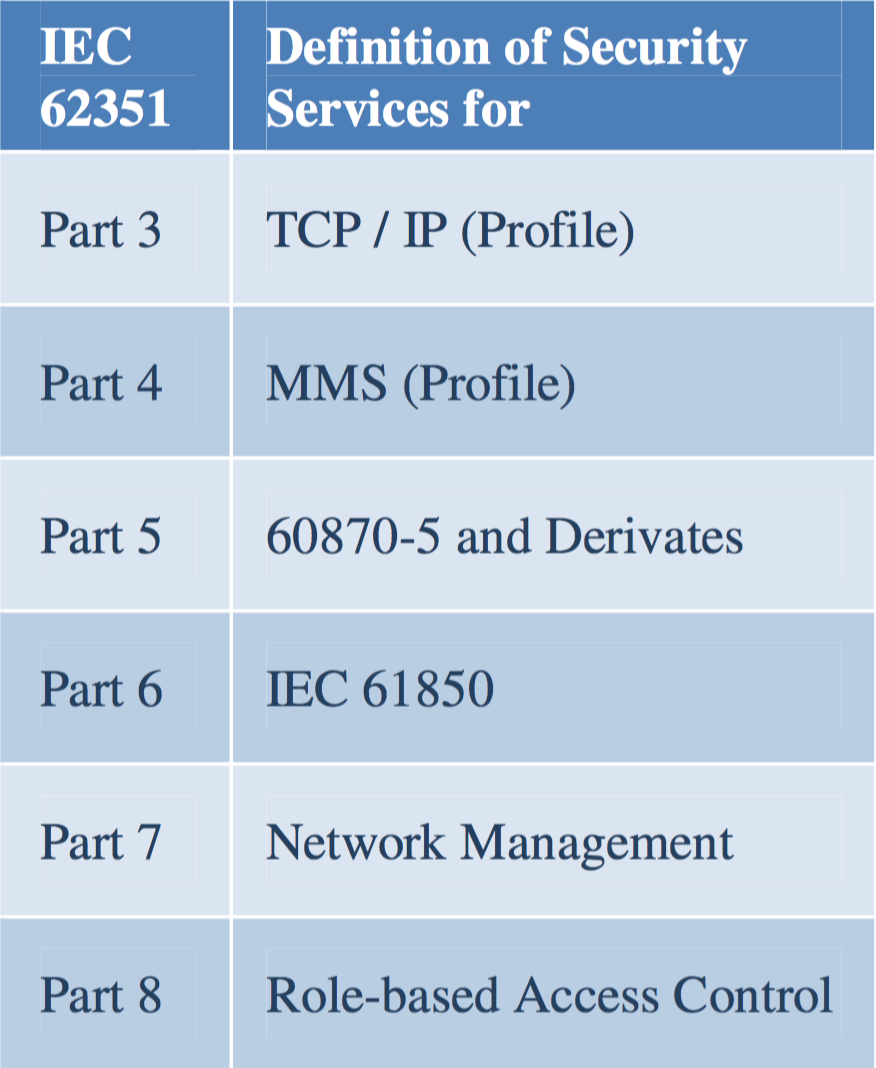
\includegraphics[scale=0.350]{imgs/62351.png}
	\caption{Overview IEC 62351} \label{fig:62351}
\end{figure}

%aggiungere soluzioni e vulnerabilità in capitolo SICUREZZA

%IEC 61850 approfondire
%IEC 62351 cita articolo e cite, aggiunta di communication tecnology (articolo troppo approfondito), meglio intro

%Citazioni
%Dopo WiMax e in dnp3
\begin{thebibliography}{99}
\bibitem{zb} ZigBee Specification, ZigBee Alliance, ZigBee Document 053474r17, January 2008.
\bibitem{tls} RFC 5246: The Transport Layer Security (TLS) Protocol, Version 1.2, T. Dierks, E Rescorla, August 2008
\end{thebibliography}